% !TEX root = main.tex
\documentclass[a4paper, UKenglish, 11pt]{uiomaster}
\usepackage{lipsum}
\usepackage[subpreambles=true]{standalone}
\usepackage[table,xcdraw]{xcolor}

\begin{document}

\chapter{Extension of the DiLoc Network}

\section{Predicting Single Dipole Sources with Amplitudes}

In the next problem, we introduce the concept of various amplitudes for single current dipole sources, which adds an additional dimension to our network's output. Besides predicting the coordinates of the dipoles for each sample, the network now also estimates the magnitude of the dipole signals. In real-world scenarios, it might be of interest to not only pinpoint the source of the abnormal activity but also comprehend the extent of abnormality. By incorporating amplitude prediction into our network, we gain valuable insights into the problem at hand and achieve a deeper understanding of the underlying brain activity.

We assign amplitudes to each dipole ranging between 1 and 10 nA$\mu$m. Although the dataset still has the same number of features, the number of target values increases by 1. Figure \ref{fig:dipole_w_amplitude_example} provides two examples from the dataset, where the dipole location remains constant while the amplitude of the dipole signal varies. In such cases, the shape of the EEG signal will remain consistent, but the magnitude of the EEG signal will be highest for the dipole with the largest amplitude.

\begin{figure}[!htb]
    \centering
    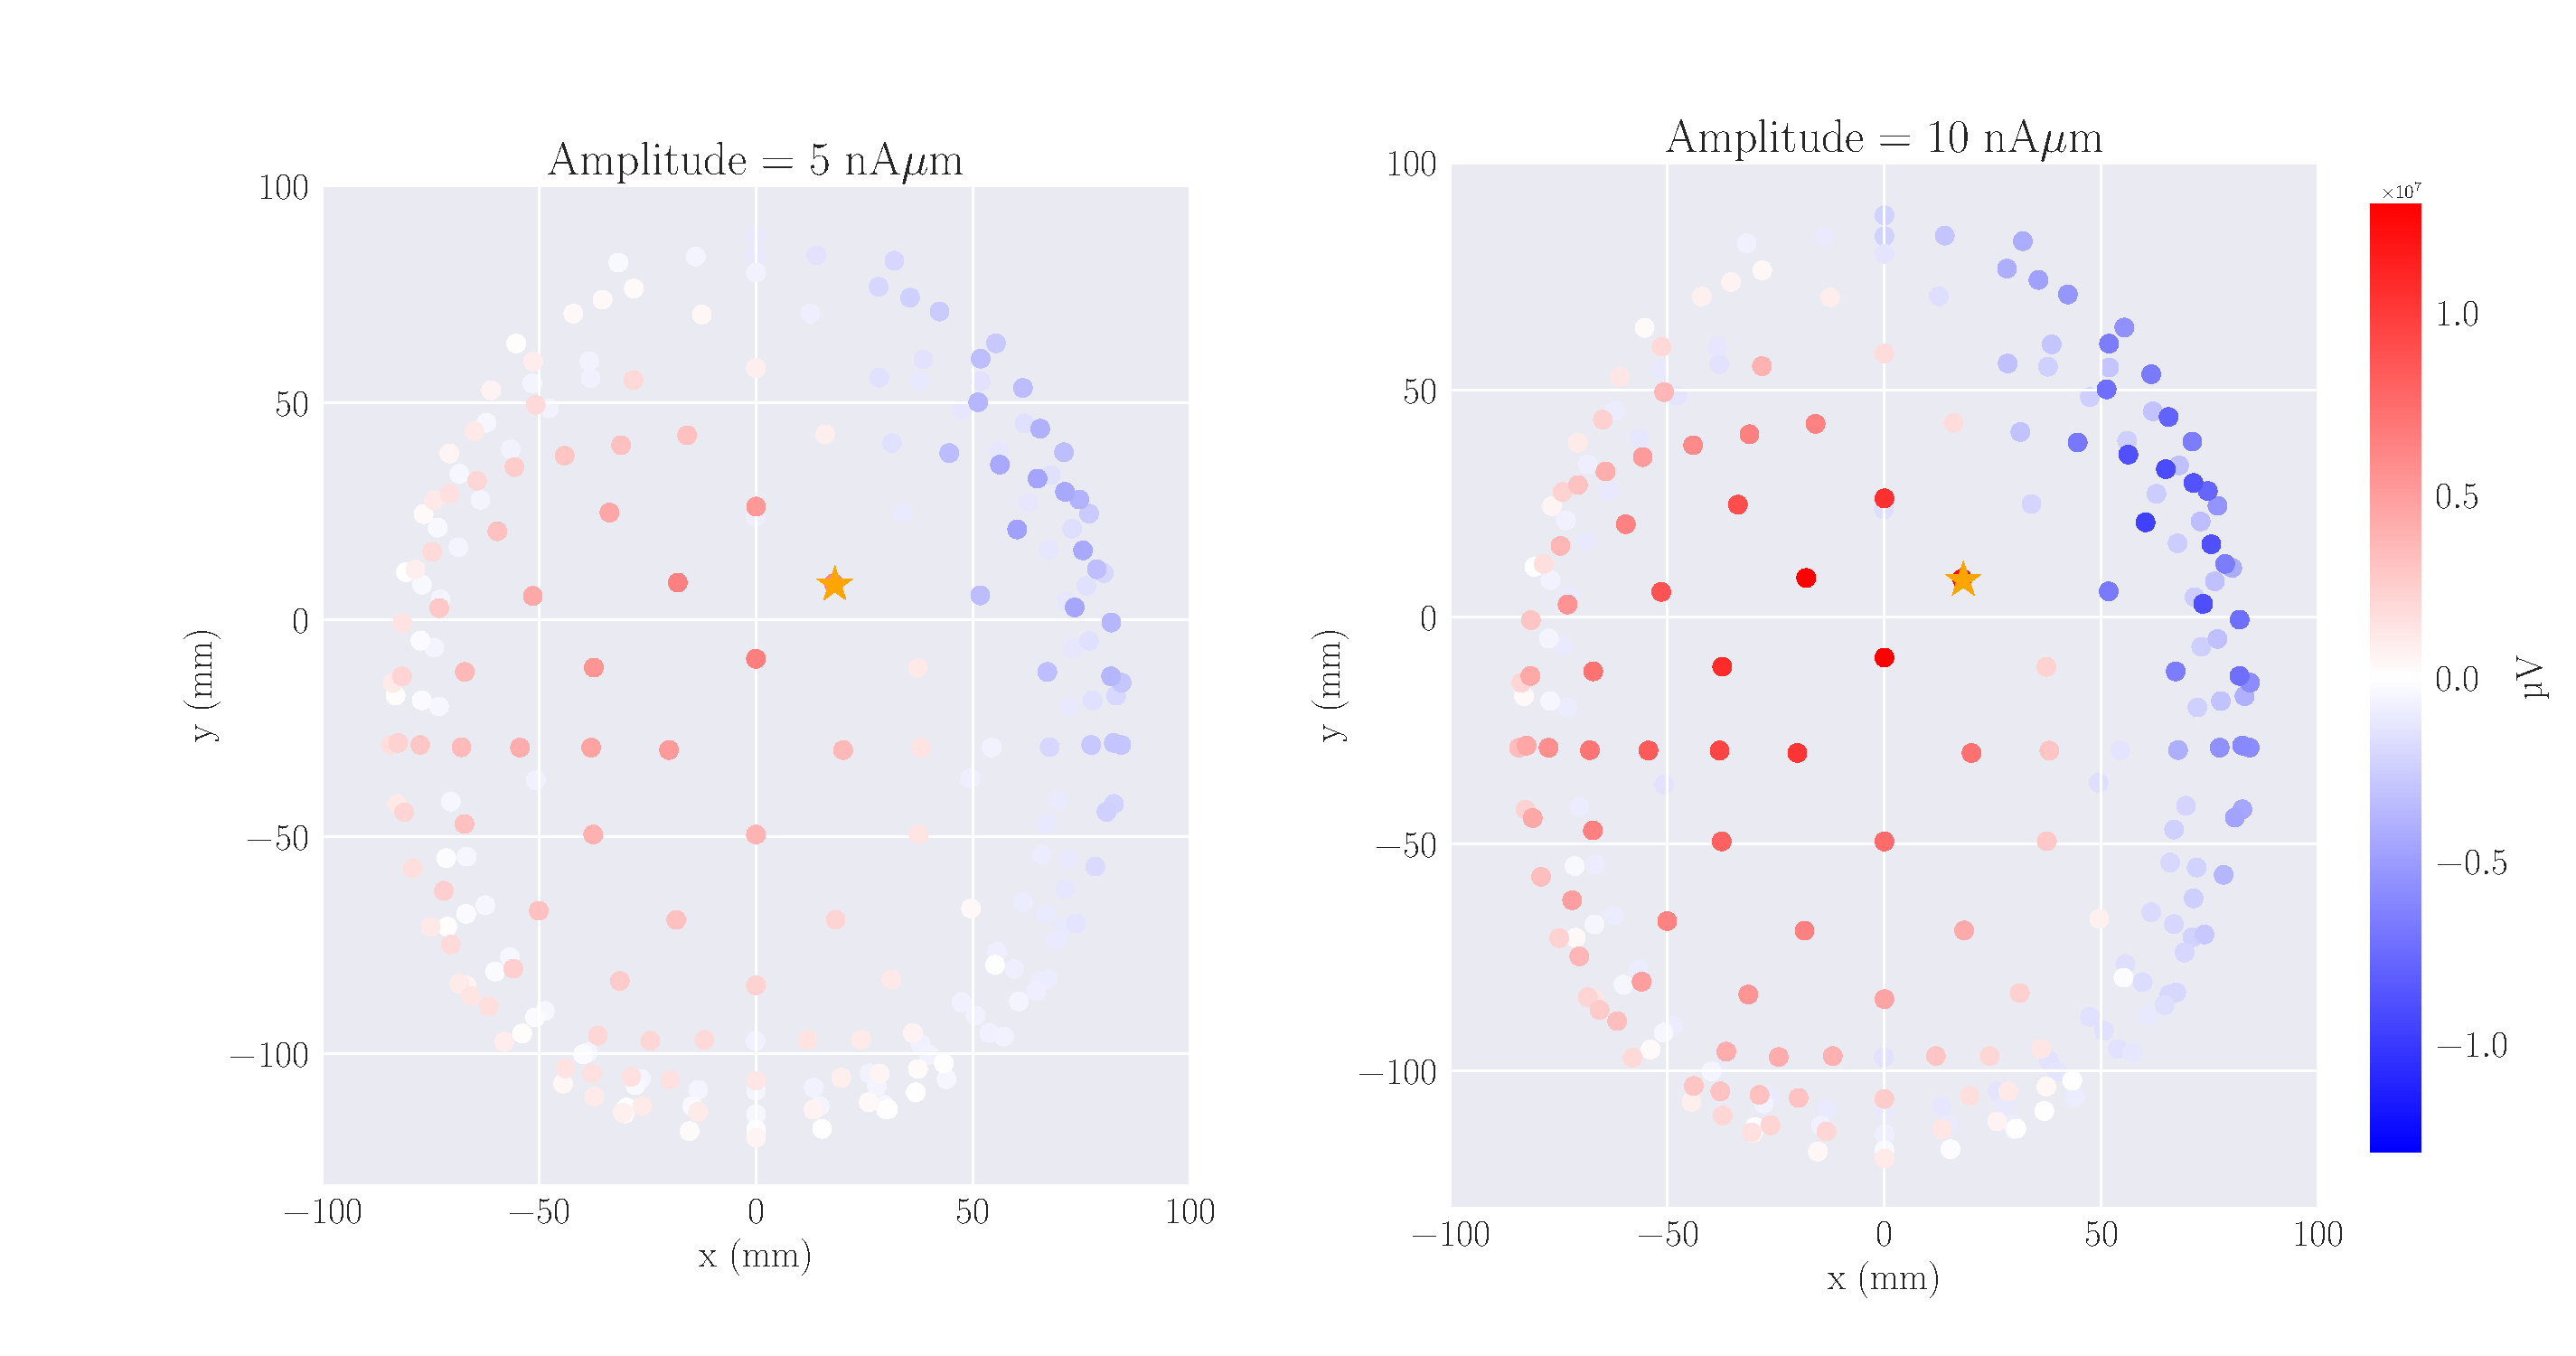
\includegraphics[width=\linewidth]{figures/dipole_w_amplitude_example.pdf}
    \caption{EEG data for two samples with current dipole amplitude equal to 5 and 10.}
    \label{fig:dipole_w_amplitude_example}
\end{figure}

We start off by introducing the extensions of out DiLoc network, that now consists of 7 hidden layers. Whereas the DiLoc neural network introduced for the purpose of localizing single current dipoles had an decreasing architecture with an increasing number of layers, the new DiLoc network now has a slightly more complicated structure. In figure \ref{fig:NN_dipole_w_amplitude_architecture} we have depiced the construction of the fully connected neural network. We see that DiLoc still takes an input of 231 data points corresponding to the number of recoring electrodes, however, the number of output nodes is increased by 1; x-coordinate, y-coordinate, z-coordinate and amplitude corresponding to the strenght of the signal for the current dipole moment in the cortex.

\begin{figure}[!htb]
    \centering
    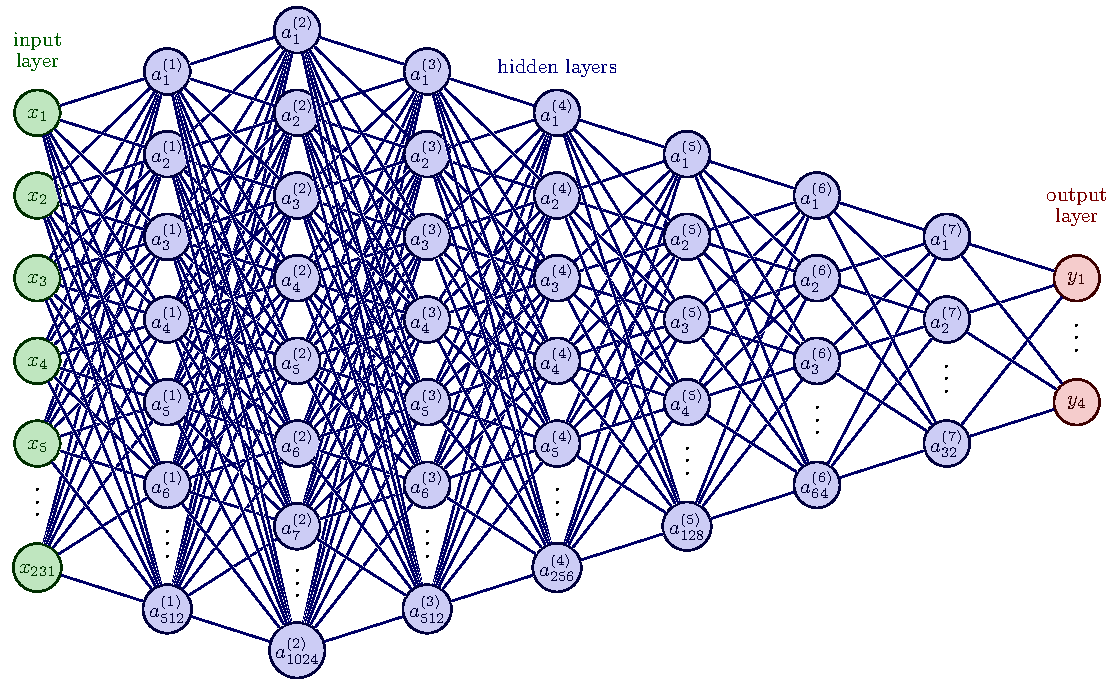
\includegraphics[width=\linewidth]{figures/NN_dipole_w_amplitude_architecture.pdf}
    \caption{Architecture.}
    \label{fig:NN_dipole_w_amplitude_architecture}
\end{figure}

In order to make the network able to genralize well and discorver the important patterns, we normalize not only the input data, but also the target data, before training. The scaling provides a set of target values ranging from 0 to 1:

\begin{equation}
    z_i = \frac{x_i - \text{min}(x)}{\text{max}(x) - \text{min}(x)}
    \label{eq:scale_target}
\end{equation}

where $z_i$ is the i$^{\text{th}}$ normalzed value in the dataset for one specific target category, $x_i$ is the i$^{\text{th}}$ value in the corresponding target data set, and min($x$) and max($x$) is the minimum and maximum value in the specific target data set. This normalization has to be done for each target category separatly. The normalization of the 4 different set of values in the target data set makes the network able to train and pick up on patterens using only one cot function. Without any form of normalization, using only one single cost function for a set of different target values with different units would not be possible.

In the extention of the DiLoc network, we continue using ReLU as activation function in the first layer, and furter the hyperbolic tangent for the hidden layers. However, as we have normalozed the output data to range from 0 to 1, it is now appropriate to utilize the Sigmoid activation function in the output layer. This activation function maps the output values to a value between 0 and 1, which is simply what we want (making the training process faster and more accurate(?)). As for the simple DiLoc model, we still use the tequniqe of adaptive learing rate. In table \ref{table:parameters} we have provided the different parameters used in the model.

% \usepackage[table,xcdraw]{xcolor}
% \usepackage[table,xcdraw]{xcolor}
\begin{table}[]
\begin{tabular}{|lc|}
\hline
\rowcolor[HTML]{CBCEFB}
\multicolumn{2}{|c|}{\cellcolor[HTML]{CBCEFB}{\color[HTML]{000000} \textbf{DiLoc for localizing current dipoles with amplitude}}}    \\ \hline
\rowcolor[HTML]{EFEFEF}
\multicolumn{1}{|l|}{\cellcolor[HTML]{EFEFEF}\textbf{Hyperparameters}} & \multicolumn{1}{l|}{\cellcolor[HTML]{EFEFEF}\textbf{Value}} \\ \hline
\multicolumn{1}{|l|}{Hidden layers}                                    & 6                                                           \\ \hline
\multicolumn{1}{|l|}{Optimizer}                                        & SGD                                                         \\ \hline
\multicolumn{1}{|l|}{Learning rate (initial)}                          & 0.001                                                       \\ \hline
\multicolumn{1}{|l|}{Momentum}                                         & 0.35                                                        \\ \hline
\multicolumn{1}{|l|}{Weight decay}                                     & 0.1                                                         \\ \hline
\multicolumn{1}{|l|}{Minibatch size}                                   & 64                                                          \\ \hline
\multicolumn{1}{|l|}{Epochs}                                           & 1000                                                        \\ \hline
\multicolumn{1}{|l|}{Dropout}                                          & 0.5                                                         \\ \hline
\end{tabular}
\end{table}
\label{tab:parameters}
\end{table}

To assess the network's performance, we analyze the accuracy in relation to training epochs, as depicted in Figure \ref{fig:dipole_w_amplitude_loss}. It is important to note that the target values have been normalized, resulting in a unitless loss measurement. Therefore, the figure provides a qualitative representation of the network's training progress rather than precise loss values. The plot clearly demonstrates a consistent pattern of decreasing loss as the number of epochs increases, indicating that the network effectively captures the underlying data patterns. Moreover, both the training and validation loss stabilize after approximately 2000 epochs, suggesting that the network may have reached its optimal performance level. In Figure \ref{fig:dipole_w_amplitude_targets}, we present the loss development for different target values. Once again, we observe that the loss stabilizes at around 2000 epochs. Notably, for the x-, z-, and y-coordinates, the stabilized loss corresponds to the minimum value reached during the training period. However, for the amplitude target value, this is not the case. From the provided figure, it is apparent that the smallest loss value occurs in a sharp dip just before reaching 500 epochs. This observation implies that if we solely aimed to minimize the loss function with respect to the amplitude value, the most optimal model would have emerged by terminating the training process at that epoch. However, since our objective is to develop a model that accurately predicts both the location and amplitude of the current dipole, we strive to train the model until the total loss is minimized, encompassing both aspects.

\begin{figure}[!htb]
    \centering
    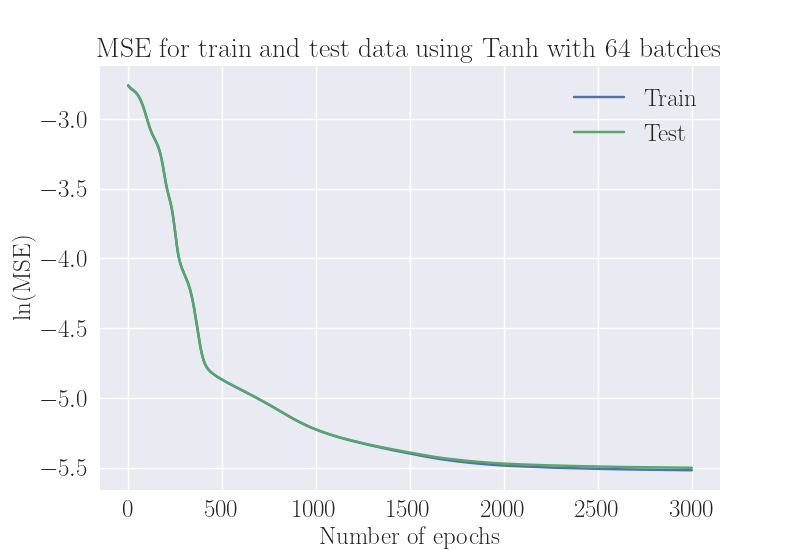
\includegraphics[width=\linewidth]{figures/MSE_tanh_50000_3july_mseloss_MSE_dipole_w_amplitude_3000_SGD_lr0.001_wd0.1_mom0.35_bs64_Tanh_64_3000_N_dipoles_1.png}
    \caption{The loss for the extended DiLoc network with 50 000 samples and hyperbolic tangent activation function.}
    \label{fig:dipole_w_amplitude_loss}
\end{figure}

\begin{figure}[!htb]
    \centering
    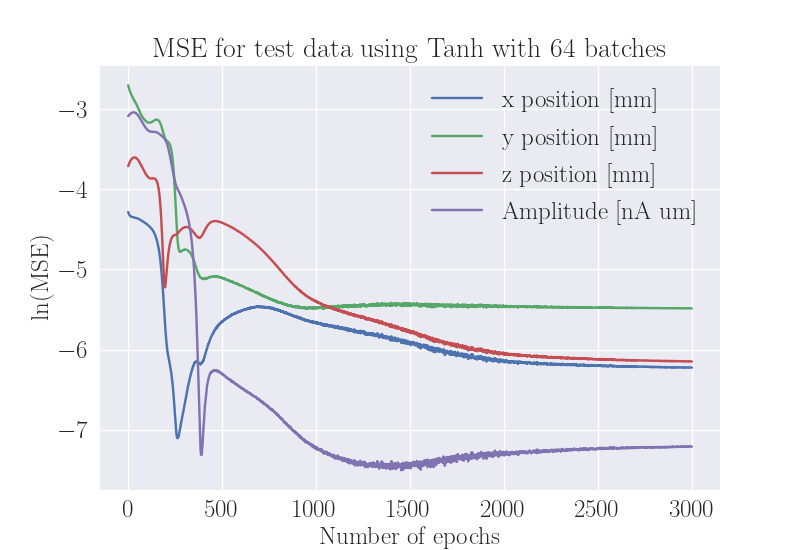
\includegraphics[width=\linewidth]{figures/mse_targets_tanh_50000_3july_mseloss_MSE_dipole_w_amplitude_3000_SGD_lr0.001_wd0.1_mom0.35_bs64.png}
    \caption{The loss developmnent for the different target values as function of epochs.}
    \label{fig:dipole_w_amplitude_targets}
\end{figure}

In Table \ref{table:error_simple_dipole} we have provided the performance of the network by concidering different error metrics. The mean absolute error (MAE) values for the x-, y-, and z- coordinates rnage from 0.8300 mm to 0.8998 mm. This means that, on average, the network's predictions have an error smaller than 1 mm in each coordinate. Considering the range of the coordinates, the MAE values represent a reasonable level of accuracy. The mean squared error penalizes larger errors/outliers more severely than MAE since it involves squaring the differences. In our case the MSE values for the different coordinates range from 1.2134 mm to 1.4110 mm. The hugher MSE values suggest that the predictions of the network may have larger errors in some cases, resulting in a higher average squared difference. However, the magnitude of the mean squared errors is still whithin a reasonable range when analyzing them in the context of the coordinates ranges. Finally the root mean squared error provides a measure of the standard deviation of the errors and helps to understand the spread of errors around the mean. The RMSE values of ours are slighly lower than the corresponding MSE values with a range from 1.1016 mm to 1.1878 mm. The table also presents the error metrics calculated for the euclidean distance. For both MAE, MSE and RMSE the value is higher than the individual coordinate errors, indicating that the errors in the x, y, and z coordinates are not perfectly aligned and contribute to the overall distance. It is worth mentioning that specific points in the cortex matrix may potentially contribute more to the errors. Further investigation could be performed to identify any specific patterns or regions in the cortex that exhibit higher error rates. However, overall the results indicate that the network is able to predict the dipole location with reasonable accuracy. While there are some errors in the predictions, the errors are generally within an acceptable range.

% Please add the following required packages to your document preamble:
% \usepackage[table,xcdraw]{xcolor}
% If you use beamer only pass "xcolor=table" option, i.e. \documentclass[xcolor=table]{beamer}
\begin{table}[!htb]
\begin{tabular}{l|
>{\columncolor[HTML]{FFFFFF}}c
>{\columncolor[HTML]{FFFFFF}}c
>{\columncolor[HTML]{FFFFFF}}c
>{\columncolor[HTML]{FFFFFF}}c
>{\columncolor[HTML]{FFFFFF}}c |}
\cline{2-6}
                                                   & \multicolumn{5}{c|}{\cellcolor[HTML]{CBCEFB}\textbf{Error for different target values}}                                                                                                                                                                                                                                                                                                                                                                                                                                                                                            \\ \cline{2-6}
                                                   & \multicolumn{1}{l|}{\cellcolor[HTML]{EFEFEF}\begin{tabular}[c]{@{}l@{}}x-coordinate\\ {[}mm{]}\end{tabular}} & \multicolumn{1}{l|}{\cellcolor[HTML]{EFEFEF}\begin{tabular}[c]{@{}l@{}}y-coordinate\\ {[}mm{]}\end{tabular}} & \multicolumn{1}{l|}{\cellcolor[HTML]{EFEFEF}\begin{tabular}[c]{@{}l@{}}z-coordinate\\ {[}mm{]}\end{tabular}} & \multicolumn{1}{l|}{\cellcolor[HTML]{EFEFEF}\begin{tabular}[c]{@{}l@{}}Euclidean \\ Distance {[}mm{]}\end{tabular}} & \multicolumn{1}{l|}{\cellcolor[HTML]{EFEFEF}\begin{tabular}[c]{@{}l@{}}Amplitude\\ {[}nA$\mu$m{]}\end{tabular}} \\ \hline
\multicolumn{1}{|l|}{\cellcolor[HTML]{EFEFEF}MAE}  & \multicolumn{1}{c|}{\cellcolor[HTML]{FFFFFF}3.627}                                                           & \multicolumn{1}{c|}{\cellcolor[HTML]{FFFFFF}4.006}                                                           & \multicolumn{1}{c|}{\cellcolor[HTML]{FFFFFF}3.476}                                                           & \multicolumn{1}{c|}{\cellcolor[HTML]{FFFFFF}2.949}                                                                  & 0.687                                                                                                           \\ \hline
\multicolumn{1}{|l|}{\cellcolor[HTML]{EFEFEF}MSE}  & \multicolumn{1}{c|}{\cellcolor[HTML]{FFFFFF}22.595}                                                          & \multicolumn{1}{c|}{\cellcolor[HTML]{FFFFFF}28.128}                                                          & \multicolumn{1}{c|}{\cellcolor[HTML]{FFFFFF}22.006}                                                          & \multicolumn{1}{c|}{\cellcolor[HTML]{FFFFFF}18.410}                                                                 & 0.687                                                                                                           \\ \hline
\multicolumn{1}{|l|}{\cellcolor[HTML]{EFEFEF}RMSE} & \multicolumn{1}{c|}{\cellcolor[HTML]{FFFFFF}4.753}                                                           & \multicolumn{1}{c|}{\cellcolor[HTML]{FFFFFF}5.306}                                                           & \multicolumn{1}{c|}{\cellcolor[HTML]{FFFFFF}4.691}                                                           & \multicolumn{1}{c|}{\cellcolor[HTML]{FFFFFF}4.291}                                                                  & 0.938                                                                                                           \\ \hline
\end{tabular}
\caption{\textbf{Evaluation of the network performance utializing different Error Metrics.} \newline
Performance for the extended DiLoc network on test dataset consisting of 1000 samples. The errors are measured using Mean Squared Error (MSE), Mean Absolute Error (MAE), and Root Mean Squared Error (RMSE).}
\label{table:error_simple_dipole}
\end{table}



\section{Predicting Region of Active Correlated Current Dipoles with Amplitudes}

In order to further enhance the complexity of our problem, we introduce jet another extension to the DiLoc neural network. By incorporating varying radii and amplitudes for the origins that generate the electrical activity detected by the recording electrodes we transforms the objective of the DiLoc network. This transforms the objective of the DiLoc network from predicting the location of individual current dipole moments to estimating the centers of larger spherical populations. This extension is valuable for the case of real-life scenarios where understanding the extent of brain damage causing abnormal activity of damaged areas may be of interest. Training the DiLoc network on such complex data, we aim to enhance its ability to generalize and serve well to real-world clinical cases.

% How we make the data

\begin{figure}[!htb]
    \centering
    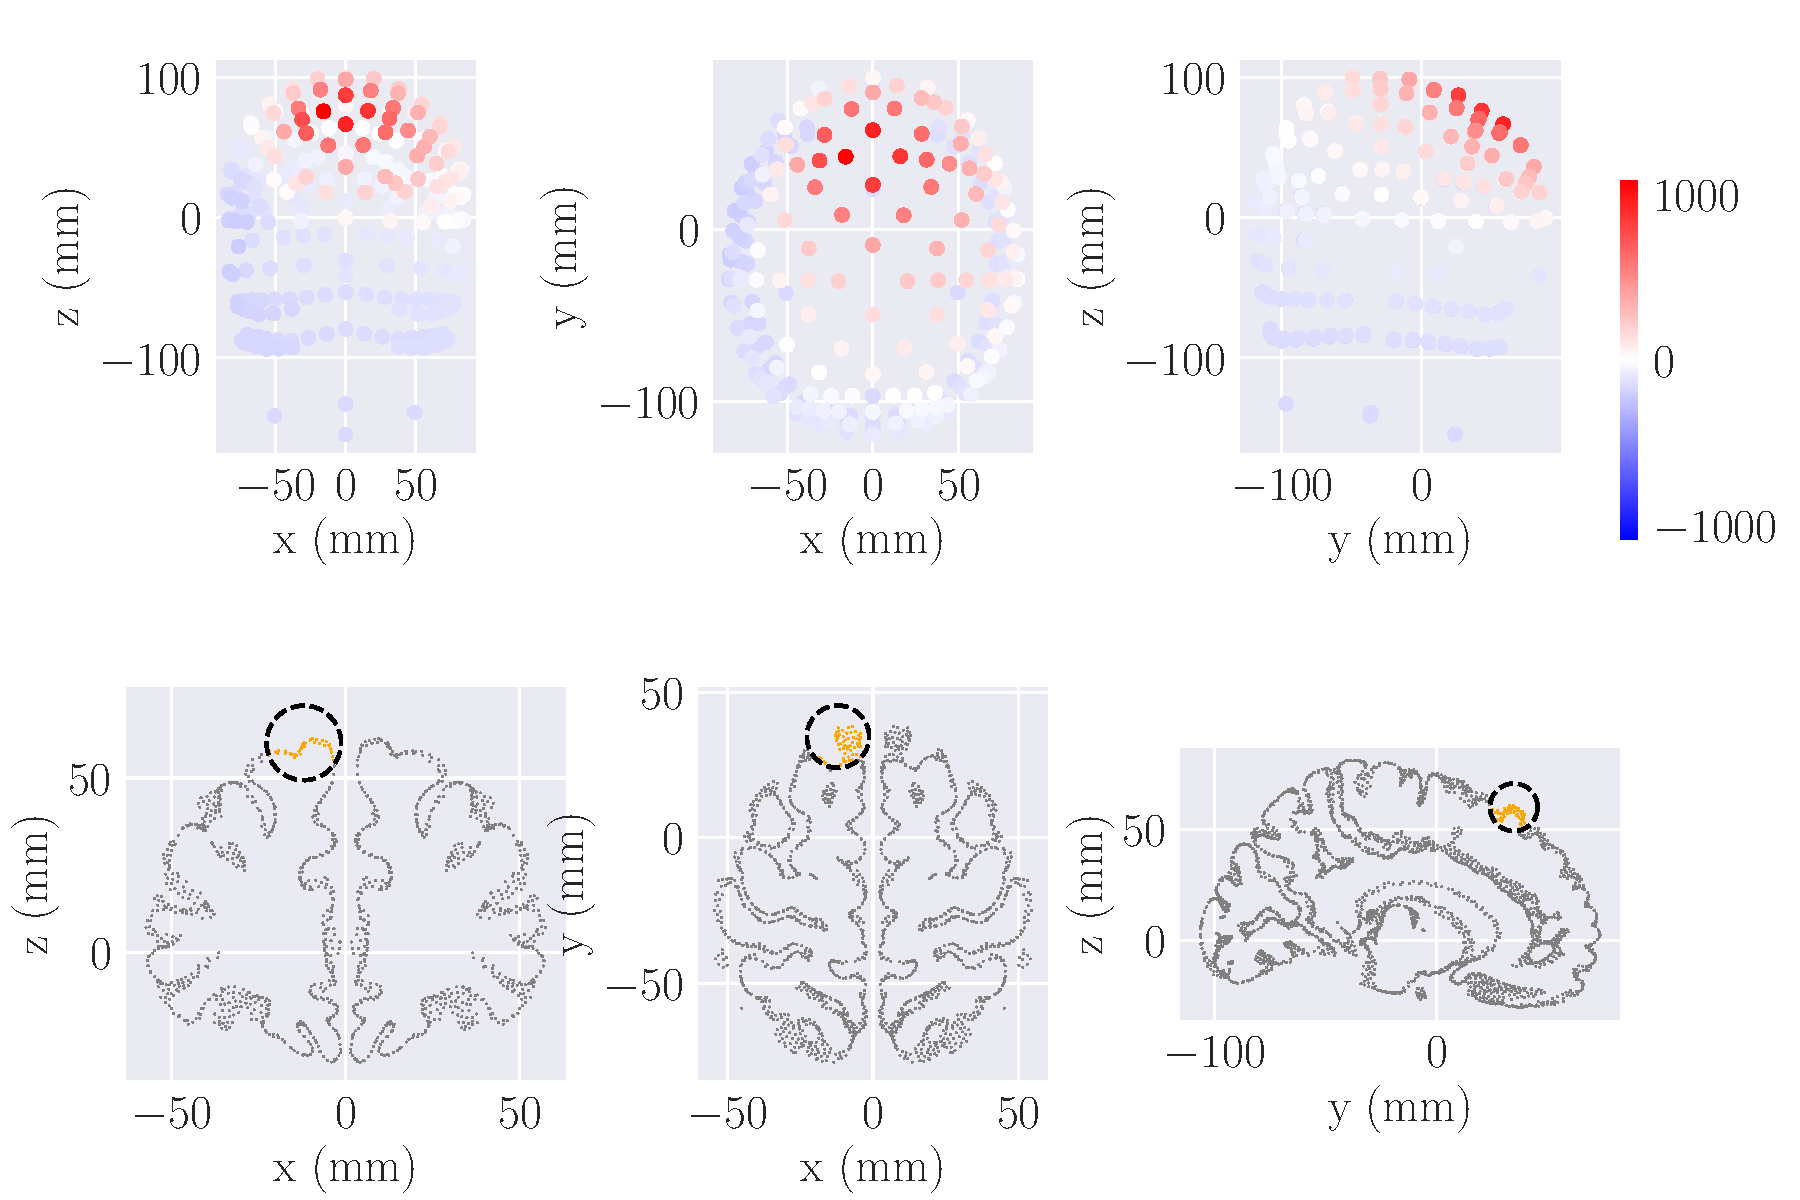
\includegraphics[width=\linewidth]{figures/dipole_area_reduced_0.pdf}
    \caption{EEG for a sample containing a spherical population of current dipole sources with a random center within the celebral cortex. The EEG measure is seen from both sides (x-, z-plane and y-, z-plane) and above (the x-, y-plane). EEG electrode locations are presented as filled circels, where the color of the fill represents the amplitude of the measured signal for the given electrode.}
    \label{fig:dipole_area}
\end{figure}

\begin{figure}[!htb]
    \centering
    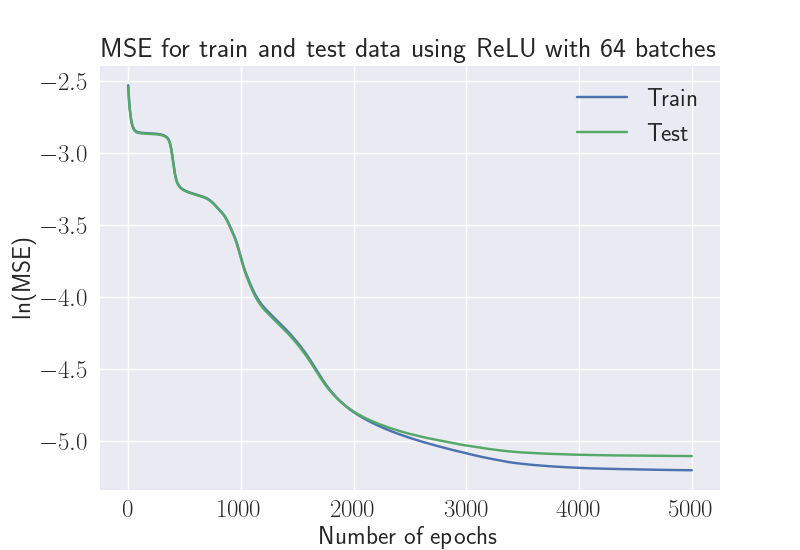
\includegraphics[width=\linewidth]{figures/MSE_50000_26junemseloss_MSE_area_w_amplitude_5000_SGD_lr0.001_wd0.1_mom0.35_bs64_ReLU_64_5000_N_dipoles_1.png}
    \caption{The validation accuracy for the simple Feed Forward Neural Network, predicting both center and radius for 50 000 samples, for 5000 epochs, with a learning rate equal to 0.001.}
    \label{fig:dipole_area_result}
\end{figure}

\begin{figure}[!htb]
    \centering
    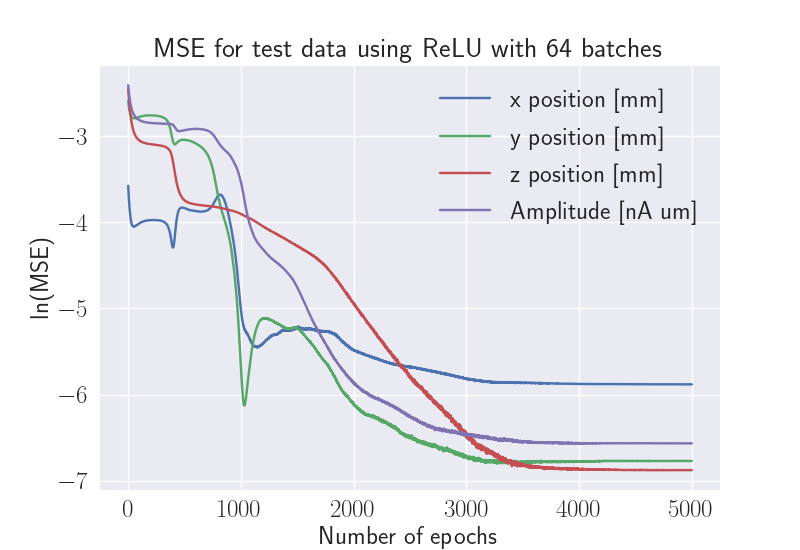
\includegraphics[width=\linewidth]{figures/mse_targets_50000_26junemseloss_MSE_area_w_amplitude_5000_SGD_lr0.001_wd0.1_mom0.35_bs64.png}
    \caption{The validation accuracy for the simple Feed Forward Neural Network, predicting both center and radius for 10 000 samples, for 10000 epochs, with a learning rate equal to 0.001.}
    \label{fig:dipole_area_result}
\end{figure}





\section{Localizing Multiple Dipole Sources}
\begin{figure}[!htb]
    \centering
    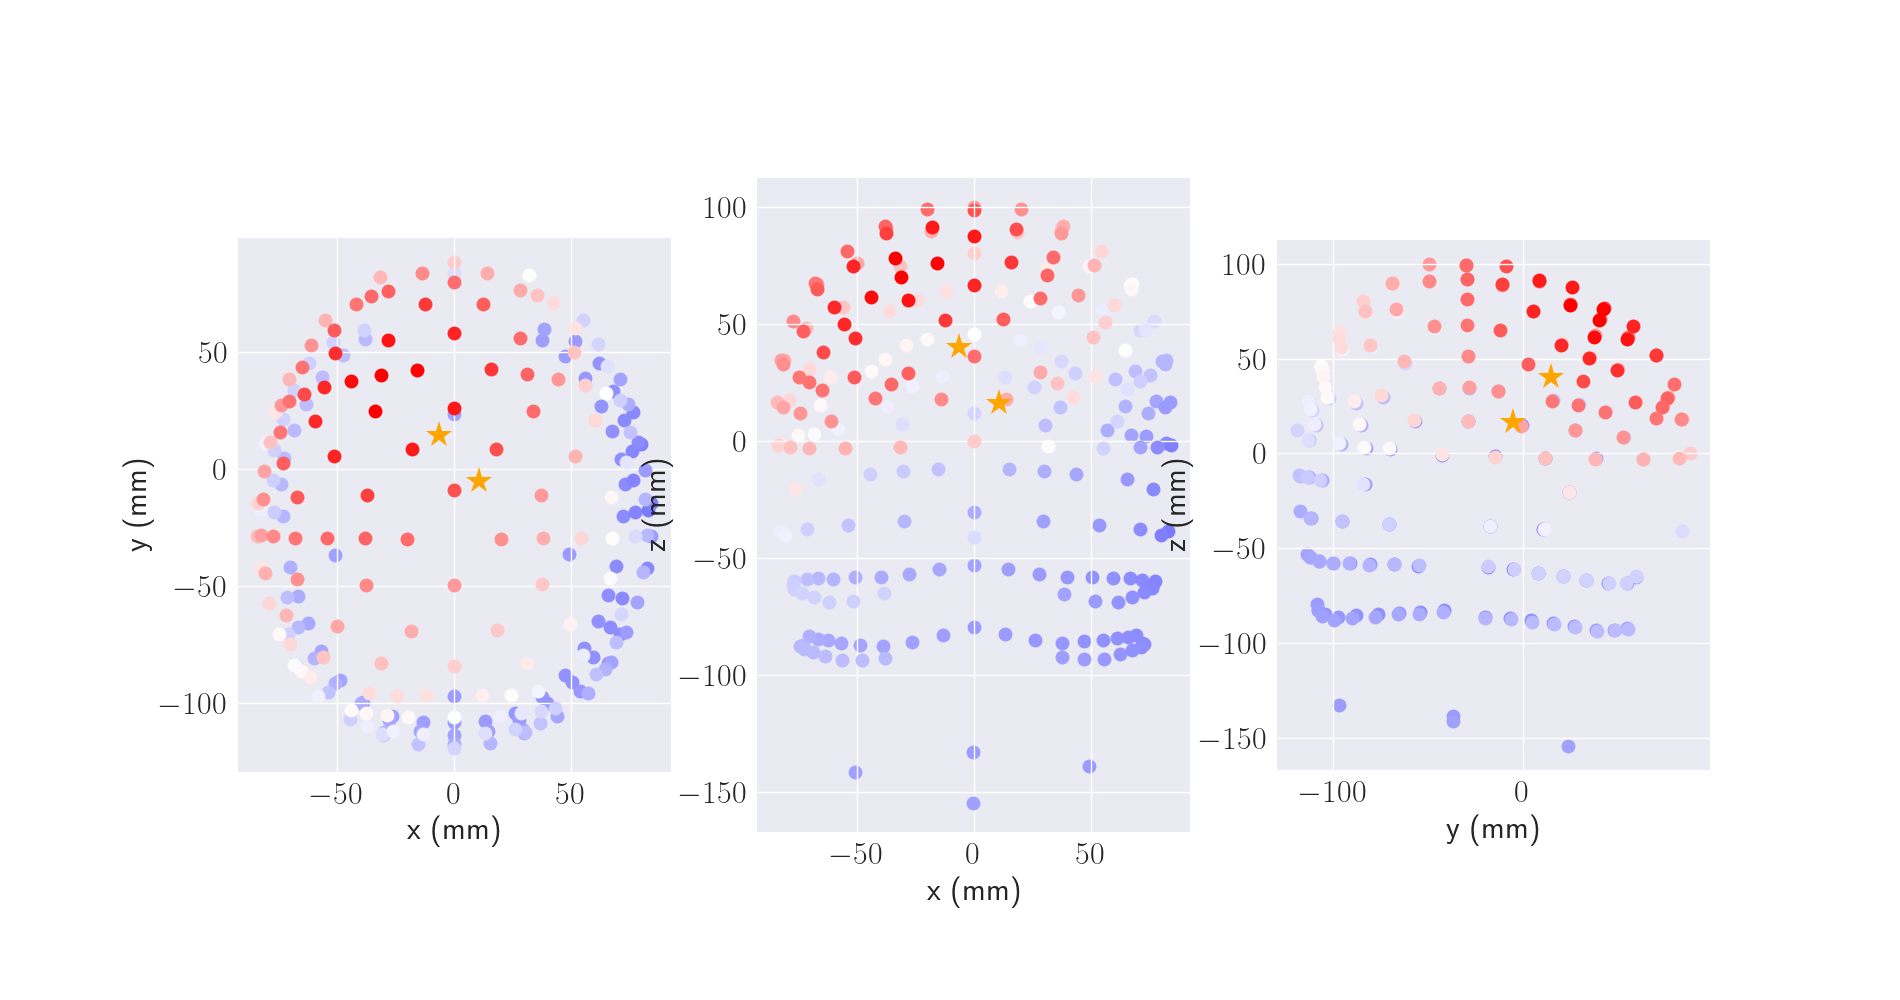
\includegraphics[width=\linewidth]{../Code/plots/finals/eeg_field_2_2.png}
    \caption{EEG for a sample containing two current dipole sources at random positions within the celebral cortex. The EEG measure is seen from both sides (x-, z-plane and y-, z-plane) and above (the x-, y-plane). EEG electrode locations are presented as filled circels, where the color of the fill represents the amplitude of the measured signal for the given electrode. The positions of the current dipole moments are marked with yellow stars.}
    \label{fig:dipole_area_result}
\end{figure}

\begin{figure}[!htb]
    \centering
    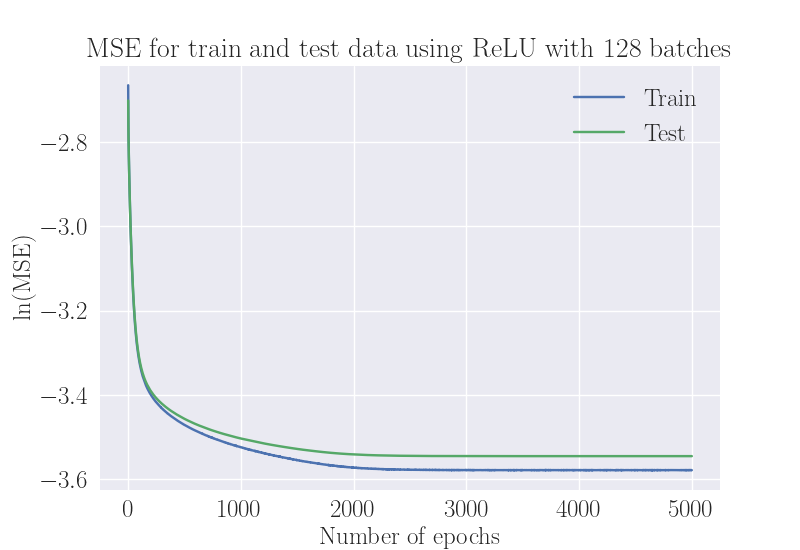
\includegraphics[width=\linewidth]{figures/MSE_26june_two_dipoles_w_amplitude_5000_SGD_lr0.001_wd0.1_mom0.35_bs128_10noise_ReLU_128_5000_N_dipoles_2.png}
    \caption{The validation accuracy for the simple Feed Forward Neural Network, predicting two current dipole sources.}
    \label{fig:dipole_area_result}
\end{figure}

\end{document}
